% !TEX root = ../main.tex
% --+ 10.31 CEBAF +-------------------------------------------------------------
\begin{frame}{Continuous Electron Beam Accelerator Facility (CEBAF)}
    \label{10.31::cebaf}

    \begin{itemize}
        \item
            \ef{CEBAF} is the linear particle accelerator housed at \ef{JLab}.

        \item
            By recirculating an $e^-$ beam in two 1.4-km-long linear accelerators, a \ef{beam energy of $\sim12$} \efe{GeV} is achieved.

        \item
            The high energy $e^-$ beam provides the ideal environment for DIS studies.
    \end{itemize}

    \begin{center}
        \begin{figure}[t]
            \centering{
                \fbox{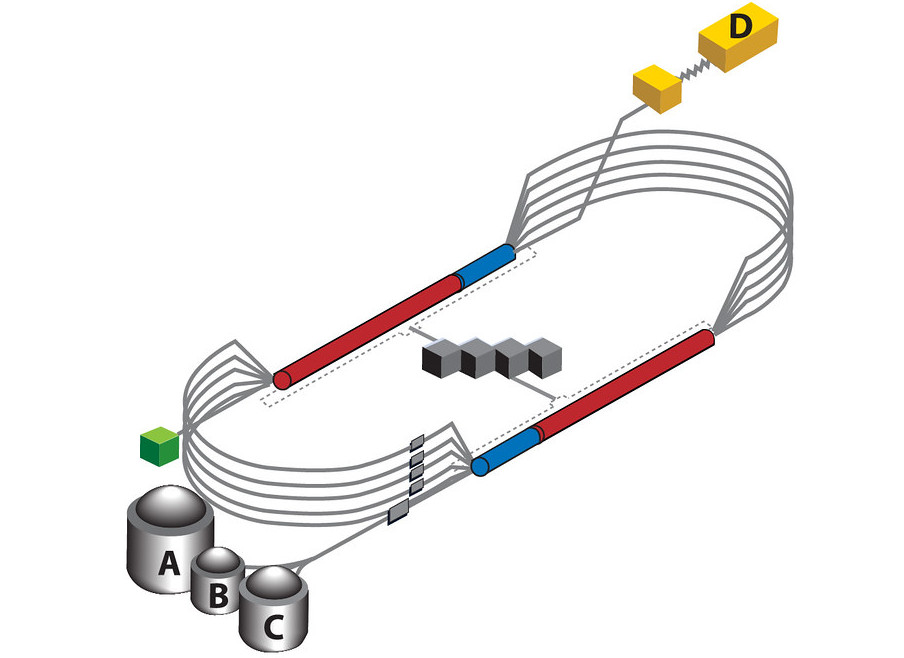
\includegraphics[width=0.5\textwidth]{31cebaf.jpg}}
            }

            \scriptsize{\textit{
                \ef{CEBAF diagram}.
                The two linear accelerators and experiment halls A to D are pictured.
            }}
        \end{figure}
    \end{center}
\end{frame}

% --+ 10.32 CLAS12 +------------------------------------------------------------
\begin{frame}{CEBAF Large Acceptance Spectrometer for 12 GeV (CLAS12)}
    \label{10.32::clas12}

    \begin{itemize}
        \item
            \ef{CLAS12} is the main particle detector at Hall B.

        \item
            The spectrometer is based on two magnets: a 3.6 T solenoid and a 5 T torus.

        \item
            The CLAS12 Forward Detector (FD) has a \ef{polar coverage from $5\degree$ to $35\degree$} and \ef{full azimuthal coverage}.
    \end{itemize}

    \vspace{-12pt}
    \begin{columns}[onlytextwidth,T]

    \begin{column}{.59\linewidth}
        \begin{center}
            \begin{figure}[t]
                \centering{
                    \fbox{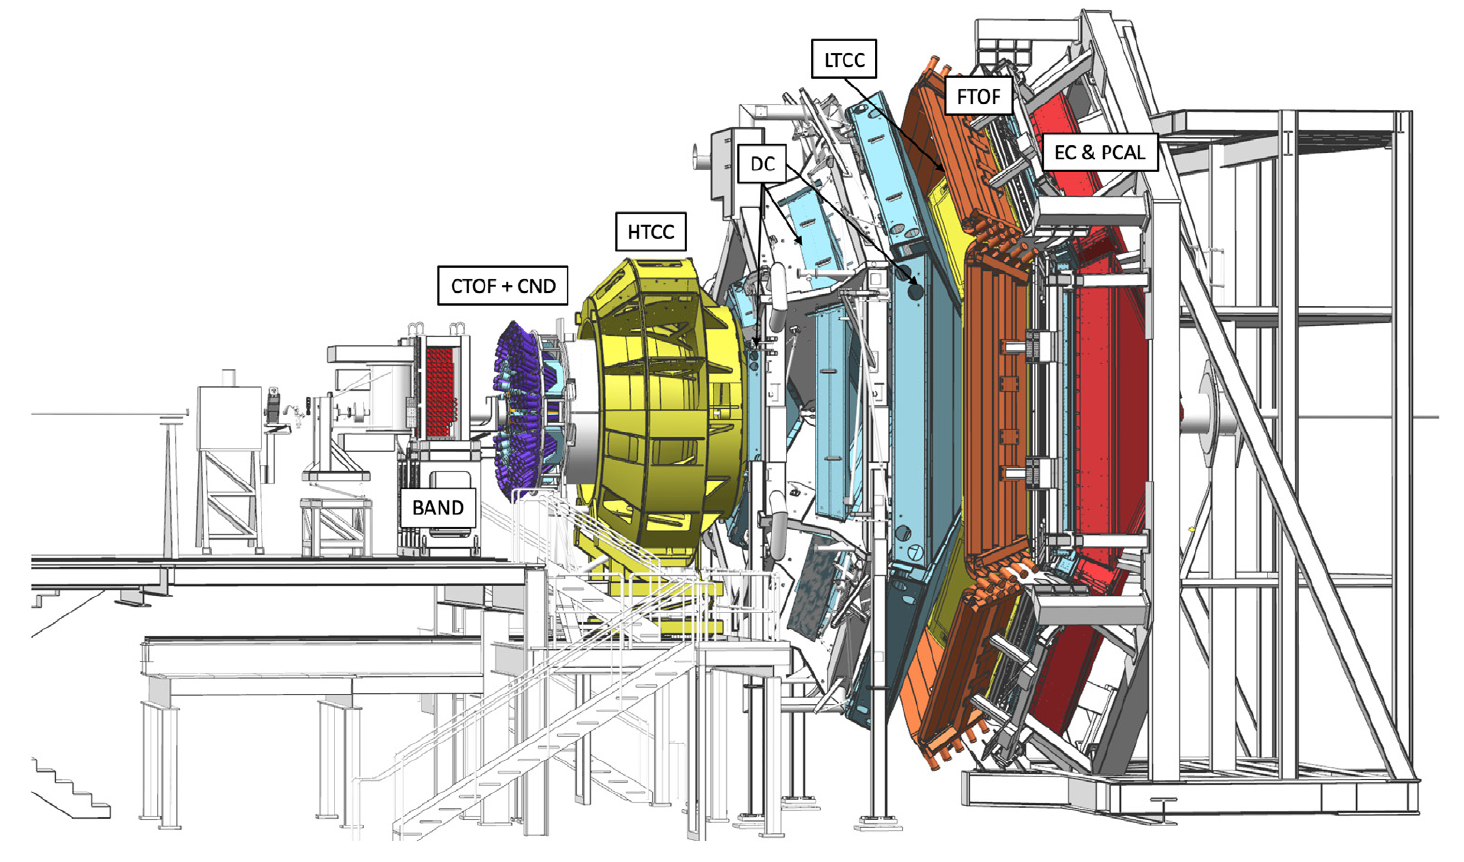
\includegraphics[width=\textwidth]{32clas12.png}}
                }
            \end{figure}
        \end{center}
    \end{column}

    \begin{column}{.39\linewidth}
        \vspace{18pt}
        \small{\textit{
            \ef{CLAS12 diagram}.
            \begin{itemize}
                % \vspace{6pt}
                % \item
                %     \ef{BAND}, \ef{CTOF}, and \ef{CND} are not used in this study.
                \vspace{6pt}
                \item
                    \ef{HTCC}, \ef{LTCC}, and \ef{FTOF} are used in particle identification and event time measurement.
                \vspace{6pt}
                \item
                    \ef{EC} and \ef{PCAL} are the forward calorimeters.
                \vspace{6pt}
                \item
                    \ef{DC} and \ef{FMT} are the forward particle trackers.
            \end{itemize}
        }}
    \end{column}

    \end{columns}
\end{frame}

% --+ 10.33 DC +----------------------------------------------------------------
\begin{frame}{Drift Chambers (DC)}
    \label{10.33::dc}

    \begin{columns}[onlytextwidth,T]

    \begin{column}{.43\linewidth}
        \vspace{36pt}
        \begin{itemize}
            \item
                The DC are the main trackers in the FD.

            \vspace{12pt}
            \item
                They use an array of HV wires to detect \ef{ionising particles}.

            \vspace{12pt}
            \item
                The particle's track is reconstructed from these signals.
        \end{itemize}
    \end{column}

    \begin{column}{.55\linewidth}
        \vspace{-12pt}
        \begin{figure}[t]
            \centering{
                \fbox{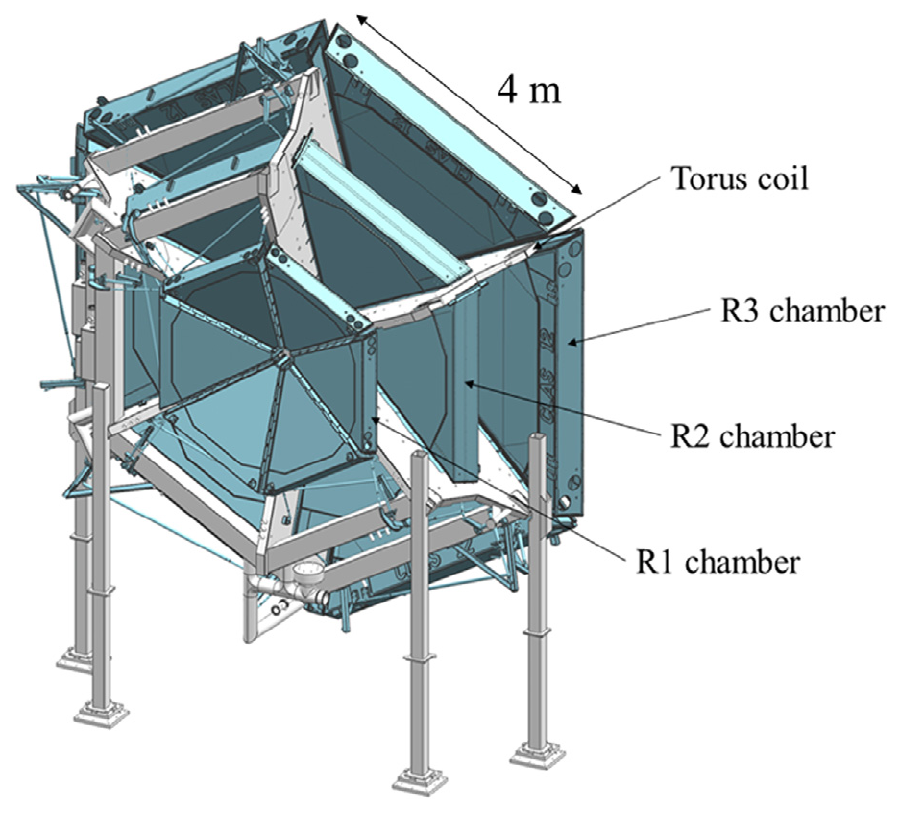
\includegraphics[width=\textwidth]{33dc.png}}
            }
        \end{figure}
        \vspace{-21pt}
        \scriptsize{\textit{
            \ef{3D render of the DC}.
            Three independent drift chambers are installed for each of the six sectors of the torus magnet.
        }}

        % \small{\textit{
        %     \ef{3d render of the DC}.
        %     Three independent drift chambers are installed for each of the six sectors.
        %     \begin{itemize}
        %         \vspace{6pt}
        %         \item
        %             Three independent drift chambers are installed in each of the six sectors of the torus magnet.
        %         \vspace{6pt}
        %         \item
        %             Each sector contains a total of \ef{36 DC layers}, each with \ef{112 sense wires}.
        %         \vspace{6pt}
        %         \item
        %             Momentum resolution: $\Delta p/p < 0.5\%$.
        %         \vspace{6pt}
        %         \item
        %             Polar resolution: \ef{$\Delta\theta < 2$} \textcolor{efd_green}{mrad}.
        %         \vspace{6pt}
        %         \item
        %             azimuthal resolution: \ef{$\Delta\phi < 2$} \textcolor{efd_green}{mrad}.
        %     \end{itemize}
        % }}
    \end{column}

    \end{columns}
\end{frame}

% --+ 10.34 FMT +---------------------------------------------------------------
\begin{frame}{Forward Micromegas Tracker (FMT)}
    \label{10.34::fmt}

    \begin{columns}[onlytextwidth,T]

    \begin{column}{.50\linewidth}
        \vspace{-12pt}
        \begin{figure}[t]
            \centering{
                \fbox{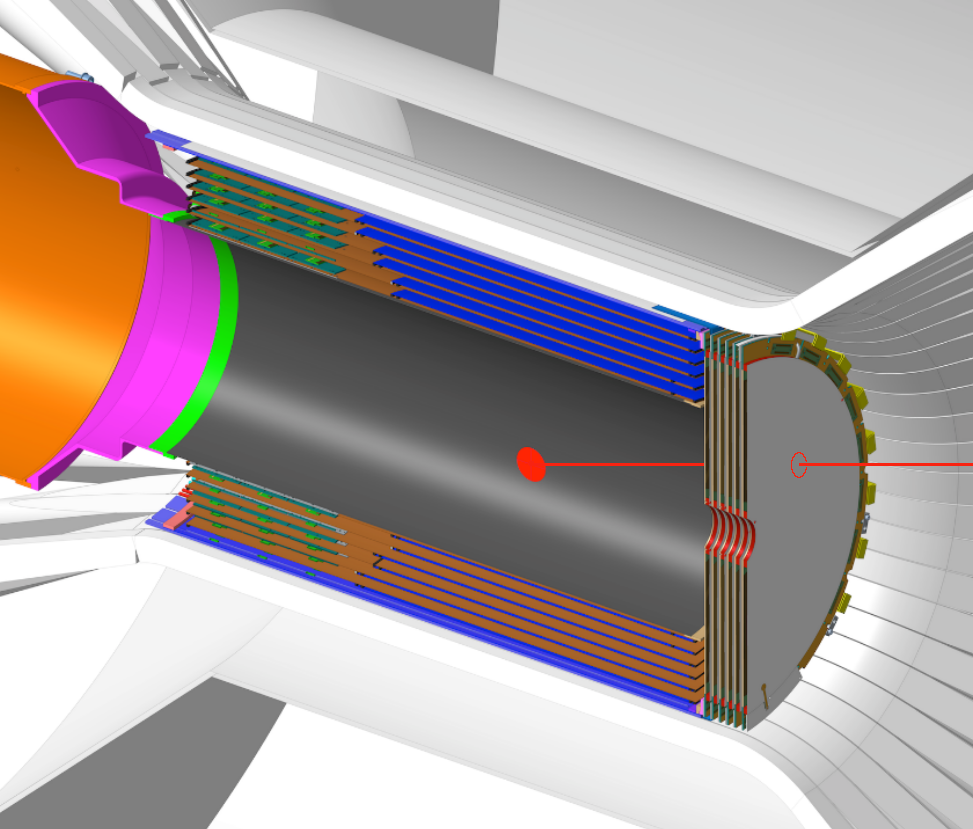
\includegraphics[width=\textwidth]{34mvt_geometry.png}}
            }
        \end{figure}
        \vspace{-21pt}
        \scriptsize{\textit{
            \ef{3D render of FMT}.
            The red dot denotes $z=0$.
            The red line denotes an arbitrary track crossing FMT.
        }}

    \end{column}

    \begin{column}{.48\linewidth}
        \vspace{24pt}
        \begin{itemize}
            \item
                FMT is a tracking detector which works in tandem with the DC.

            \vspace{12pt}
            \item
                It uses micromegas tracking technology\appref{20.01::micromegas_tracking} to detect \ef{ionising particles}.

            \vspace{12pt}
            \item
                FMT has \ef{3 layers}\appref{20.02::fmt_geometry}.
                The first sits at \ef{$z \approx 26$} \textcolor{efd_green}{cm}.
        \end{itemize}
    \end{column}

    \end{columns}
\end{frame}
